
%----------------------------------------------------------------------------------------
%	PART
%----------------------------------------------------------------------------------------


\part{Anexos}
\graphicspath{ {C_Capitulo_Anexos/img/ejemplos/}, {W_Varios/2_Portada_capitulos} }



%----------------------------------------------------------------------------------------
%	PART
%----------------------------------------------------------------------------------------

\chapterimage{C_Capitulo_Anexos/img/portada/ima2} % Chapter heading image


\chapter{Anexos}
\section{Capítulo 1}

\begin{spacing}{1.5}
 La fórmula de valor futuro es la suma entre el valor presente y el interés simple \ref{eq1}, la definición de interés simple  redefine la formula en general, teniendo en cuenta que el interés simple es la multiplicación entre el valor presente, la tasa de interés periódico y el periodo. Reescribimos la formula remplazando el interés simple, luego factorizamos la variable del valor presente y de esta manera obtenemos otra forma de hallar el valor futuro.
 \begin{center}
  \begin{align*}
   F & = P+I\hspace{40 pt} \textit{Fórmula inicial de Valor Futuro } \\
   I & = Pin\hspace{40 pt} \textit{Fórmula de interés simple}        \\
   F & = P+Pin\hspace{40 pt} \textit{Remplazando formulas}           \\
   F & = P(1+in)\hspace{40 pt} \textit{Fórmula final Valor Futuro}
  \end{align*}
 \end{center}
 La fórmula de Valor liquido es la diferencia entre el valor futuro y el descuento, de la misma manera la fórmula del valor de descuento depende de la tasa anticipada, un valor futuro y un periodo de tiempo. Remplazando en la formula inicial y factorizando el valor futuro redefinimos la formula, como lo muestra el siguiente procedimiento matemático.
 \clearpage
 \begin{align*}
  D  & = Fdn\hspace{40 pt} \textit{Fórmula de valor descuento }       \\
  VL & = F-D\hspace{40 pt} \textit{Fórmula inicial de Valor Liquido } \\
  VL & = F-(Fdn)\hspace{40 pt} \textit{Remplazando formulas}          \\
  VL & = F(1-dn)\hspace{40 pt}\textit{Fórmula final Valor Liquido}
 \end{align*}
 Una de las demostraciones más importantes en este capítulo, es la referenciada al descuento por fidelidad, se simplifica cuando se entiende que no se suman unos descuentos con otros. %, por tanto, en la siguiente tabla se muestra el proceso para demostrar la formula.
 %\begin{center}
 %\begin{table}[H]
 %\fontsize{11}{9}\selectfont
 %\centering
 %\begin{tabular}{@{}|c|c|c|c|@{}}
 %\toprule
 %\textbf{\begin{tabular}[c]{@{}c@{}}Valor de la Factura\\ antes del Descuento\\ {[}F{]}\\ (1)\end{tabular}} & %\textbf{\begin{tabular}[c]{@{}c@{}}Tasa de \\ Descuento\\ {[}d{]}\\ (2)\end{tabular}} & \textbf{\begin{tabular}[c]{@{}c@{}}Valor del\\ %Descuento\\ {[}D=Fd{]}\\ (3)\end{tabular}} & \textbf{\begin{tabular}[c]{@{}c@{}}Valor de la factura\\ después del descuento\\ {[}P = F-D = F %- F  d{]}\\ (4)\end{tabular}} \\ \midrule
 %F                                  & $d_1$                              & $Fd_1$                             & $F-Fd_1 = F(1-%d_1)$                \\
 %$F(1-d_1)$                         & $d_2$                              & $F(1-d_1)d_2$                      & %\begin{tabular}[c]{@{}c@{}}$F(1-d_1) - F(1-d_1)d_2 = F(1-d_1)(1-d_2)$\end{tabular}
 %\\
 %$F(1-d_1)(1-d_2)$                  & $d_3$                              & $F(1-d_1)(1-d_2)d_3$               & %\begin{tabular}[c]{@{}c@{}}$F(1-d_1)(1-d_2)-F(1-d_1)(1-d_2)d_3 =  F(1-d_1)(1-d_2)(1-d_3)$\end{tabular}          \\
 %|                                  & |                                  & |                                  & %|                                  \\
 %|                                  & |                                  & |                                  & %|                                  \\
 %|                                  & |                                  & |                                  & %|                                  \\
 %|                                  & |                                  & |                                  & %|                                  \\

 %\begin{tabular}[c]{@{}c@{}}$F(1-d_1)(1-d_2)...(1-d_{n-1})$  \end{tabular}          & $d_n$                              & %\begin{tabular}[c]{@{}c@{}}$F(1-d_1)(1-d_2)...(1-d_{n-1})d_n$  \end{tabular}
 %                                   & $F(1-d_1)(1-d_2)...(1-%d_n)$                                                                                  \\ \bottomrule
 %\end{tabular}
 %\end{table}
 %\end{center}
 Primero se comienza definiendo el valor de la factura antes del primer descuento en este caso es F, la tasa de descuento d1 y el valor del descuento D1, luego nos dan el valor de la factura después del descuento, que en si solo es la formula de valor presente de un flujo futuro.
 \newline
 Lo que se puede hacer es explicar paso por paso lo que la tabla nos quiere demostrar, para ello partimos de las siguientes premisas:
 \clearpage
 \begin{center}
  \begin{align*}
   F     & = F \hspace{140 pt}\textit{Valor Factura inicial}                              \\
   D_1   & = Fd_{1}\hspace{130 pt} \textit{Valor del Descuento 1 }                        \\
   P_1   & = F-D_{1}\hspace{118 pt} \textit{Valor Presente de un flujo futuro}            \\
   P_1   & = F-(Fd_{1})\hspace{103 pt} \textit{Remplazando en la fórmula}                 \\
   P_1   & = F(1-d_{1})\hspace{105 pt}\textit{Fórmula factura final con el descuento 1}   \\
   \newline
   F_{2} & = P_{1} \hspace{138 pt}\textit{Valor Factura inicial 2}                        \\
   D_{2} & = F_{2}d_{2}\hspace{128 pt} \textit{Valor del Descuento 2 }                    \\
   D_{2} & = F(1-d_{1})d_{2}\hspace{95 pt} \textit{Reemplazando el valor de P }           \\
   P_{2} & = F_{2}-D_{2}\hspace{113 pt} \textit{Valor Presente de un flujo futuro}        \\
   P_{2} & = F(1-d_{1})-F(1-d_{1})d_{2} \hspace{40 pt} \textit{Remplazando en la fórmula} \\
   P_{2} & = F(1-d_{1})[1-d_{2}]\hspace{71 pt}\textit{Factorizando F}                     \\
  \end{align*}
 \end{center}
 Repitiendo el procedimiento anterior, al final obtenemos la formula n-ésima.
 \begin{center}
  $D=F(1-d_{1} )(1-d_{2} )...(1-d_{n})$
 \end{center}
\end{spacing}
\clearpage
\section{Capítulo 2}

\begin{spacing}{1.5}

 $F = P(1+i)^n$  \hspace{35pt}  \textit{Valor futuro}\\

 Algebraicamente podemos representar el resultado anterior en la siguiente forma:\\

 \begin{table}[H]
  \centering
  \begin{tabular}{@{}|c|c|c|c|@{}}
   \toprule
   \textbf{\begin{tabular}[c]{@{}c@{}}Periodo\\ (n)\\ {[}1{]}\end{tabular}} & \textbf{\begin{tabular}[c]{@{}c@{}}Capital Inicial \\ (P)\\ {[}2{]}\end{tabular}} & \textbf{\begin{tabular}[c]{@{}c@{}}Interés\\ (I)\\ {[}3{]}\end{tabular}} & \textbf{\begin{tabular}[c]{@{}c@{}}Capital Final\\ (F)\\ {[}4{]}\end{tabular}}             \\ \midrule
   0                                  & 0                                  & 0                                  & $F_0 = P$                                      \\
   1                                  & P                                  & Pi                                 & $F_1 = P + Pi = P(1+i)      $                  \\
   2                                  & P(1+i)                             & P(1+i)i                            & $F_2 = P(1+i)+P(1+i)i=P(1+i)^2$                \\
   3                                  & $P(1+i)^2 $                        & $P(1+i)^{2}i $                     & $F_3 = p(1+i)^{2}+P(1+i)^{2}i=P(1+i)^{3} $     \\
   4                                  & $P(1+i)^{3}$                       & $P(1+i)^{3}i$                      & $F_4 = p(1+i)^{3}+P(1+i)^{3}i=P(1+i)^{4}$      \\
   .                                  & .                                  & .                                  & .                                              \\
   .                                  & .                                  & .                                  & .                                              \\
   .                                  & .                                  & .                                  & .                                              \\
   n                                  & $P(1+i)^{n-1}$                     & $P(1+i)^{n-1}i$                    & $F_n = P(1+i)^{n-1}+P(1+i)^{n-1}i=P(1+i)^{n} $ \\ \bottomrule
  \end{tabular}
 \end{table}

 con lo que llegamos a concluir que la formula del interes compuesto es:\\
 $F = (1+i)^n$\\
 Donde:
 \\
 F = \hspace{32pt}  \textit{Valor final o monto}\\
 i = \hspace{35pt}  \textit{Tasa interes periodico vencido} \\
 n = \hspace{34pt}  \textit{Número  de periodos}\\   % 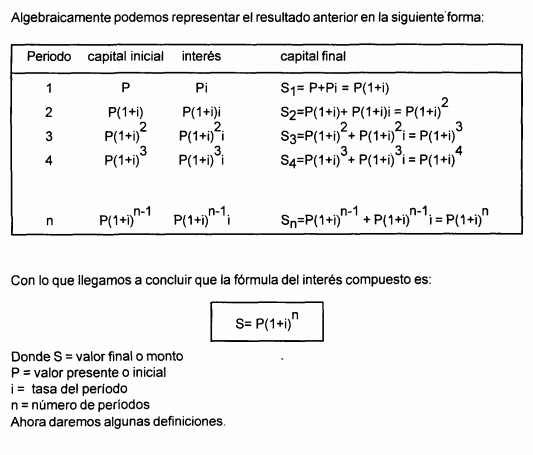
\includegraphics[height = 8 cm]{valorFuturo}\\
 j = im \hspace{23pt}  \textit{Tasa nominal anual}\\
 La tasa nominal anual es igual a la tasa de interes periodico vencido multiplicada por el numero de periodos que hay en un año, el numero de periodos que hay en un año lo representamos por m, asi llegamos a la formula anterior.\\


\end{spacing}

\section{Capítulo 6}

\begin{itemize}
 \item La fórmula del valor de un flujo n-ésimo se representa de la siguiente forma:

       \vspace{4mm}

       $R_{n}=R_{1} + (n-1)L$ \hspace{35 pt} \textit{Valor último flujo de un gradiente aritmético}\\

       En donde se puede ver que el valor n-ésimo del flujo esta dado por el primer flujo al que se le suman el valor del gradiente aritmético monetario multiplicado por el número de periodos menos uno.

       \vspace{4mm}

       Si se parte de la fórmula original se tiene

       \vspace{4mm}

       $R_{n}=R_{n-1} + L$ \hspace{55 pt} \textit{Valor último flujo de un gradiente aritmético}\\

       de igual forma se sabe que

       \vspace{4mm}

       $R_{n-1}=R_{n-2} +L$ \hspace{45 pt} \textit{Valor del penúltimo flujo de un gradiente aritmético}\\

       Reemplazando se tiene

       \vspace{4mm}

       $R_{n}=R_{n-2} +2L$ \hspace{50 pt} \textit{Valor último flujo de un gradiente aritmético}\\

       \vspace{4mm}

       Si este proceso se repite n menos una, veces se obtiene lo siguiente

       \vspace{4mm}

       $R_{n}=R_{1} + (n-1)L$ \hspace{37 pt} \textit{Valor último flujo de un gradiente aritmético}\\


 \item El flujo n-ésimo de un gradiente geométrico esta dado por la siguiente fórmula

       \vspace{4mm}

       $R_{n} = R_{1}(1+g)^{n-1}$ \hspace{37 pt} \textit{Flujo n-ésimo de un gradiente geométrico}\\

       Donde el flujo n-ésimo viene dado por el valor del primer flujo, multiplicado por uno más el valor del gradiente geométrico elevado a la n menos una veces.

       \vspace{4mm}

       Por definición el flujo n-ésimo se puede escribir de la sieguiente forma:

       \vspace{4mm}

       $R_{n} = R_{n-1}(1+g)$ \hspace{44 pt} \textit{Flujo n-ésimo de un gradiente geométrico}\\

       y debido a que

       \vspace{4mm}

       $R_{n-1} = R_{n-2}(1+g)$ \hspace{31 pt} \textit{Flujo n-1 de un gradiente geométrico}\\

       Por lo que reemplazando se obtiene

       \vspace{4mm}

       $R_{n} = R_{n-2}(1+g)(1+g)$ \hspace{9 pt} \textit{Flujo n-ésimo de un gradiente geométrico}\\

       $R_{n} = R_{n-2}(1+g)^{2}$ \hspace{35 pt} \textit{Flujo n-ésimo de un gradiente geométrico}\\

       Si se realiza este proceso n menos una veces se llega a:

       \vspace{4mm}

       $R_{n} = R_{1}(1+g)^{n-1}$ \hspace{35 pt} \textit{Flujo n-ésimo de un gradiente geométrico}\\

\end{itemize}

\phantomsection
\setlength{\columnsep}{0.75cm}
\printindex





%----------------------------------------------------------------------------------------
